\documentclass{beamer}
\usepackage[mode=buildnew,subpreambles=true]{standalone}

\usepackage{pgf, tikz}
\usetikzlibrary{shapes.misc}
\usetikzlibrary{decorations.pathreplacing}

\tikzset{cross/.style={cross out, draw=black, minimum size=2*(#1-\pgflinewidth), inner sep=0pt, outer sep=0pt},
%default radius will be 1pt. 
cross/.default={0.25pt},
    point/.style={
    thick,
    draw=black,
    cross out,
    inner sep=0pt,
    minimum width=4pt,
    minimum height=4pt,
    },
}

\graphicspath{{figures/images/}{figures/figs/}}

\title{Analyse numérique de la criticalité de la transition de jamming pour des particules sphéroïdales}

\author{Yann-Edwin Keta}

\date{Stage de recherche, printemps 2017}

\begin{document}

% page de couverture

\begin{frame}

\begin{minipage}{0.2\linewidth}
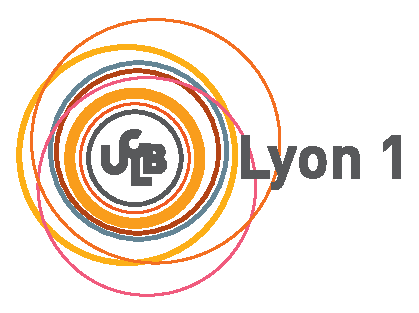
\includegraphics[scale=0.4]{logoucbl.eps}
\end{minipage}
\hfill
\begin{minipage}{0.2\linewidth}

\includegraphics[scale=0.13]{udl-logo.png}
\end{minipage}
\hfill
\begin{minipage}{0.2\linewidth}

\includegraphics[scale=0.25]{logoens.eps}
\end{minipage}
\titlepage
\begin{minipage}{\linewidth}
\begin{center}
{\small Stage encadré par~:}\\ 
\textbf{Peter OLSSON}
\end{center}
\end{minipage}

\end{frame}

% introduction
{
\makeatletter % to change template
    \setbeamertemplate{headline}[default] % not mandatory, but I though it was better to set it blank
    \def\beamer@entrycode{\vspace*{-\headheight}}
\begin{frame}{Introduction}

\begin{itemize}
\item Milieux granulaires
    \begin{itemize}
    \item[$\rightarrow$] présents presque partout, 2e matériau le plus manipulé dans l’industrie après l’eau ;
    \item[$\rightarrow$] système non-thermique ;
	\item[$\rightarrow$] milieux relativement simples mais aux propriétés surprenantes (par exemple effet Janssen ou mémoire lors de la compaction).
    %     \begin{itemize}
	   % \item on s'intéresse ici à la transition de jamming
    %     \end{itemize}
    \end{itemize}
    \vspace{10pt}
\item Transition de jamming a été très bien étudiée depuis un peu plus de 10 ans pour des particules parfaitement sphériques
    \begin{itemize}
        \item[$\rightarrow$] moins pour des particules ellipsoïdales...
    \end{itemize}
\end{itemize}

\end{frame}
}

\section{Quaternions}

\subsection{Propriétés}

\begin{frame}{Propriétés}

% Introduits par Hamilton comme extension des nombres complexes.

\begin{defi}[Quaternions]
\begin{align*}
q = q_0 + \sum_{i=1}^{3}q_i e_i\text{, avec } \begin{cases} e_m^2 = -1& \\ e_me_n = \varepsilon_{mnk} e_k&\text{, } m \neq n \end{cases}
\end{align*}
\end{defi}

\begin{theo}[Rotations dans l'espace]
Toute rotation dans l'espace d'un vecteur $\vec{v}$ pour donner un vecteur $\vec{v}\prime$ peut s'exprimer par l'action d'un quaternion unitaire $q$ sur ce vecteur :
\vspace{-10pt}
\begin{align*}
\vec{v'} = q\vec{v}q^* \text{, avec } \vec{v}=\begin{pmatrix}v_1\\v_2\\v_3\end{pmatrix}\equiv\sum_{i=1}^3 v_ie_i
\end{align*}
\end{theo}

$\Rightarrow$ l’orientation d’un vecteur en fonction du temps peut-être décrite par un quaternion dont les coordonnées sont des fonctions du temps

\end{frame}

\subsection{Intégration}

\begin{frame}{Conservation de l'unitarité}

$\rightarrow$ quaternions $\equiv$ vecteurs unitaires de $\mathbb{R}^4$ $\Rightarrow$ intégration sur l'hypersphère
\vspace{-10pt}

\begin{figure}[h!]
\centering
\includestandalone{figures/tikz/quaternion_numerical_integration}
\caption{Schéma de l'intégration numérique (Euler)}
\end{figure}

\end{frame}

\begin{frame}{Intégration}

$\rightarrow$ On peut montrer que l'évolution temporelle d'un quaternion décrivant l'orientation d'un vecteur fixe dans un solide est liée au vecteur vitesse angulaire par la relation
\begin{align*}
\vec{\omega}(t) = 2q^*(t)\dot{q}(t)
\end{align*}
dans la base des axes principaux du solide, permettant ainsi l'intégration du quaternion.\\
\vspace{10pt}

$\rightarrow$ Le vecteur rotation est intégré en utilisant l'équation d'Euler pour la rotation des corps non-déformables.

\end{frame}

\subsection{Intérêt}

\begin{frame}{Intérêt}

\begin{itemize}
    \item Stockés plus facilement que des matrices de rotation et plus robustes aux erreurs d'arrondis.
    \vspace{10pt}
    \item Très utilisés en aérospatial mais aussi dans la conception des animations pour jeux-vidéo.
\end{itemize}

\end{frame}

\section{Ellipsoïdes}

\subsection{Propriétés}

\begin{frame}{Matrice caractéristique}

\begin{theo}[Matrice caractéristique]
Une ellipsoïde $\mathcal{A}$ de centre $\vec{r_0}$ peut être décrite par une matrice réelle définie positive $B\equiv Q \text{diag}(R_i^{-2})_{i=1:3} Q^T$ telle que
\vspace{-10pt}
\begin{align*}
\forall \vec{r} \in \mathbb{R}^3, \begin{cases} (\vec{r} - \vec{r_0})^T B (\vec{r} - \vec{r_0}) < 1 &\text{ si } \vec{r} \in \mathcal{A} \setminus \bar{\mathcal{A}} \\ (\vec{r} - \vec{r_0})^T B (\vec{r} - \vec{r_0}) = 1 &\text{ si } \vec{r} \in \bar{\mathcal{A}} \\ (\vec{r} - \vec{r_0})^T B (\vec{r} - \vec{r_0}) > 1 &\text{ si } \vec{r} \notin \mathcal{A} \end{cases}
\end{align*}

\vspace{-10pt}
avec $Q$ la matrice de rotation de $\mathcal{A}$ et $(R_i)_{i=1:3}$ les longueurs de ses semi-axes.
\end{theo}

\begin{theo}[Facteur d'échelle]
On définit $\mu(\vec{r}\in\mathbb{R}^3)$ le facteur d'échelle à appliquer à $\mathcal{A}$ pour que $\vec{r}$ soit à sa surface. Alors :
\begin{align*}
\mu^2(\vec{r}) = (\vec{r}-\vec{r_0})^TB(\vec{r}-\vec{r_0})
\end{align*}
\end{theo}

\end{frame}

\subsection{Intersections}

\begin{frame}{Détermination de l'intersection de 2 ellipsoïdes}

Pour pouvoir déterminer les interactions entre 2 particules ellipsoïdales, il est nécessaire de savoir si elles s'intersectent.
\begin{itemize}
\item[$\rightarrow$] Perram et Werhteim (1985) ont proposé une méthode efficace pour déterminer le facteur d'échelle $\mu$ à appliquer à 2 ellipsoïdes $\mathcal{A}$ et $\mathcal{B}$ afin qu'elles soient tangentes.
\begin{itemize}
    \item[$\Rightarrow$] $\mu > 1 \Leftrightarrow \mathcal{A}\cap\mathcal{B} = \emptyset$
\end{itemize}
\item[$\rightarrow$] Implémentation numérique inspirée de Perram et Wertheim (1985) et la thèse de A. Donev (2007).
\end{itemize}

\end{frame}

\section{Transition de jamming}

\subsection{Jamming}

\begin{frame}{Phénomène}

\begin{itemize}
\item Pierre-Gilles de Gennes (1998) : "l’étude des milieux granulaires est au niveau de celle de la physique des solides en 1930" ; Leo Kadanoff (1999) : "nous pourrions réinventer la physique statistique par l’étude des milieux granulaires".
\end{itemize}

\begin{defi}[Transition de jamming]
Apparition d’une contrainte seuil dans un milieu granulaire désordonné.
\end{defi}

\begin{itemize}
\item[$\rightarrow$] Cette transition peut apparaître sous l’effet de l’augmentation de la densité $\phi$ au dessus d’une valeur critique $\phi_J$
    \begin{itemize}
    \item[$\rightarrow$] bas $\phi$ : les particules peuvent bouger indépendamment ;
    \item[$\rightarrow$] haut $\phi$ : les particules ne peuvent pas s’éviter $\Rightarrow$ apparition d'un module de flexion.
    \end{itemize}
\item[$\rightarrow$] Ce phénomène de jamming apparaît partout, de manière volontaire (e.g., pour remplacer les bras mécaniques) ou involontaire (e.g., blocage de grains dans un silo).
\end{itemize}

\end{frame}

\begin{frame}{Différentes observations}

Le phénomène de jamming est rencontré dans de nombreux systèmes sous différentes conditions expérimentales
\begin{itemize}
\item[$\rightarrow$] mousses sous l’effet de cisaillement, transition vitreuse (transformation des liquides en solides désordonnés) ;
\item[$\rightarrow$] origine commune ?
\end{itemize}

\begin{figure}[h!]
\centering
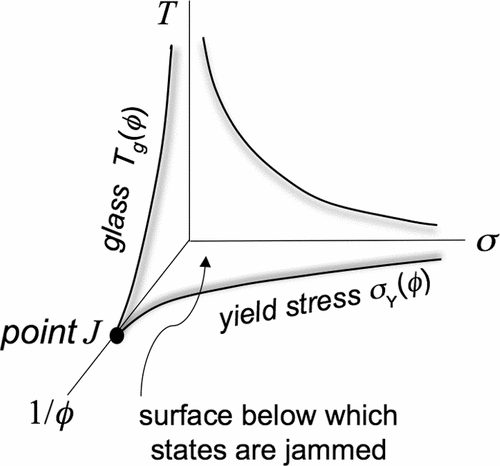
\includegraphics[width=0.28\textwidth]{figures/images/phase_diagram.png}
\caption{\textit{source:} Vågberg, Olsson, Teitel (2011)}
\end{figure}

\end{frame}

\begin{frame}{Transition étudiée}

Nous étudions nous la transition de jamming pour des systèmes athermiques ($T=0$), non soumis à une contrainte de cisaillement ($\sigma=0$), dans la limite thermodynamique d’un système infini ($N\rightarrow+\infty$)
\begin{itemize}
\item[$\rightarrow$] survient à $\phi = \phi_J$ ;
\item[$\rightarrow$] correspond à un point critique.
\end{itemize}

\end{frame}

\subsection{Exposants critiques}

\begin{frame}{Théorie du groupe de renormalisation}

La théorie du groupe de renormalisation permet par des arguments d’échelle d’étudier les états d’un système, notamment proche de points critiques
\begin{itemize}
\item[$\rightarrow$] permet d’expliquer pourquoi et comment certaines quantités divergent proche d’un point critique ;
\item[$\rightarrow$] donne une justification théorique à l’existence des exposants critiques.
\end{itemize}

\end{frame}

\begin{frame}{Divergence des coefficients de transport newtoniens}

Pour un ensemble de particules sphériques soumis à un taux de cisaillment $\dot{\gamma}$, les coefficients de transports newtoniens associés à la contrainte de cisaillement $\sigma$, $\eta\equiv\frac{\sigma}{\dot{\gamma}}$, et à la pression $p$, $\eta_p\equiv\frac{p}{\dot{\gamma}}$, divergent proche de la densité de jamming $\phi_J$ avec un exposant critique $\beta$ (Olsson et al., 2007).
\begin{align*}
\eta,\eta_p \isEquivTo{\phi\rightarrow\phi_J} (\phi_J-\phi)^{-\beta}
\end{align*}
dans la limite $\dot{\gamma}\rightarrow0$.\\
\vspace{10pt}

La pression décroît exponentiellement si le cisaillement est stoppé avec un temps caractéristique $\tau$ qui diverge aussi proche de la densité de jamming avec un exposant $\beta$ (Olsson, 2015).
\begin{align*}
\tau \isEquivTo{\phi\rightarrow\phi_J} (\phi_J-\phi)^{-\beta}
\end{align*}

\end{frame}

\begin{frame}{Comportement de la pression proche de la transition de jamming}
Inspirés de la théorie du groupe de renormalisation, nous supposons que la pression se comporte selon l'équation
\begin{align*}
p(\delta\phi,\dot{\gamma}) \sim \dot{\gamma}^{h_p} g_p^{(\text{fit})}((\phi-\phi_J)\dot{\gamma}^{q_p})
\end{align*}
proche de la transition de jamming, où $h_p$ et $q_p$ sont des inconnues vérifiant $\beta=(q_p-1)/h_p$.\\
\vspace{10pt}

Numériquement, la fonction $g^{\text{(fit)}}_p$ et les inconnues $h_p$ et $q_p$ sont déterminées par la méthode de Levenberg-Marquadt.

\end{frame}

\subsection{Modèles et méthodes}

\begin{frame}{Modèles}

\begin{itemize}
\item[$\rightarrow$] Potentiel élastique d'interaction entre 2 particules, inspiré par le modèle de Dorian pour des bulles sphériques, et appliqué à 2 ellipsoïdes $\mathcal{A}$ et $\mathcal{B}$.
\begin{align*}
\mathcal{V}_{\mathcal{A}\mathcal{B}}(\vec{r_{\mathcal{A}}},\vec{r_{\mathcal{B}}}) = \begin{cases} \frac{1}{2} k_e (1 - \mu(\vec{r_{\mathcal{A}}},\vec{r_{\mathcal{B}}}))^2 &\text{ if } \mathcal{A} \cap \mathcal{B} \neq \emptyset\\ 0 &\text{ if } \mathcal{A} \cap \mathcal{B} = \emptyset \end{cases}
\end{align*}
\item[$\rightarrow$] Modèle pour la force de dissipation identique à celui utilisé pour des particules sphériques par Olsson, en prenant en compte les rotations.
\begin{align*}
\vec{f}_{\mathcal{A}\mathcal{B}}^{\text{dis}} = -k_d(\vec{v_\mathcal{A}}^{C_\mathcal{B}} - \vec{v_\mathcal{B}}^{C_\mathcal{A}})
\end{align*}
\item[$\rightarrow$] Nous calculerons la pressions uniquement avec la force élastique.
\end{itemize}

\end{frame}

\begin{frame}{Méthodes}

\begin{itemize}
\item Les simulations correspondent à des cisaillements d’ensembles de particules sphéroïdales athermiques et molles sans interactions coulombiques.
    \begin{itemize}
	\item[$\rightarrow$] Les exposants critiques sont ensuite déterminés grâce à notre hypothèse de comportement de la pression proche de la densité de jamming ;
	\item[$\rightarrow$] l’intérêt du cisaillement est qu’il casse les amas (clusters) de particules à l’origine d’une densité $\phi_J$ mal définie dans des simulations impliquant des compressions par exemple.
	\end{itemize}
\item Les mesures du temps de relaxation se font en 2 parties : cisaillement puis relaxation.
\end{itemize}

\end{frame}

\section{Résultats}

\subsection{Transition rhéologique}

\begin{frame}{Augmentation du nombre de contact}
\vspace{-10pt}

\begin{figure}[h!]
\centering
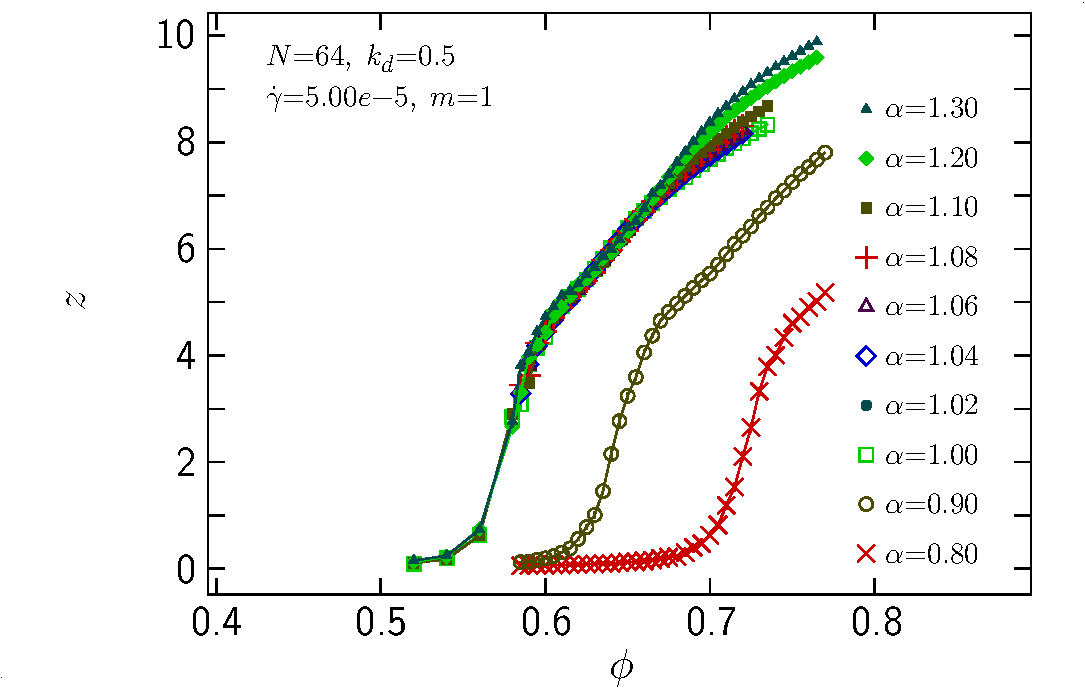
\includegraphics[width=0.6\textwidth]{figures/figs/z_phi_0064_KDk500_Ml100_GDg500}
\caption{Nombre de contacts moyen par particule en fonction de la densité pour différents rapports d'aspect $0.8\le\alpha\le1.3$. $N=64,~ k_d=0.5,~ \dot{\gamma}=5e-5,~ m=1$.}
\end{figure}

\vspace{-10pt}
Transition rhéologique caractérisée par une augmentation brusque du nombre de contacts par particules apparaissant à la même densité pour les rapports d'aspect considérés.

\end{frame}

\begin{frame}{Coefficients de transport}

\begin{figure}[h!]
\centering
    \begin{subfigure}[t]{0.49\textwidth}
        \centering
        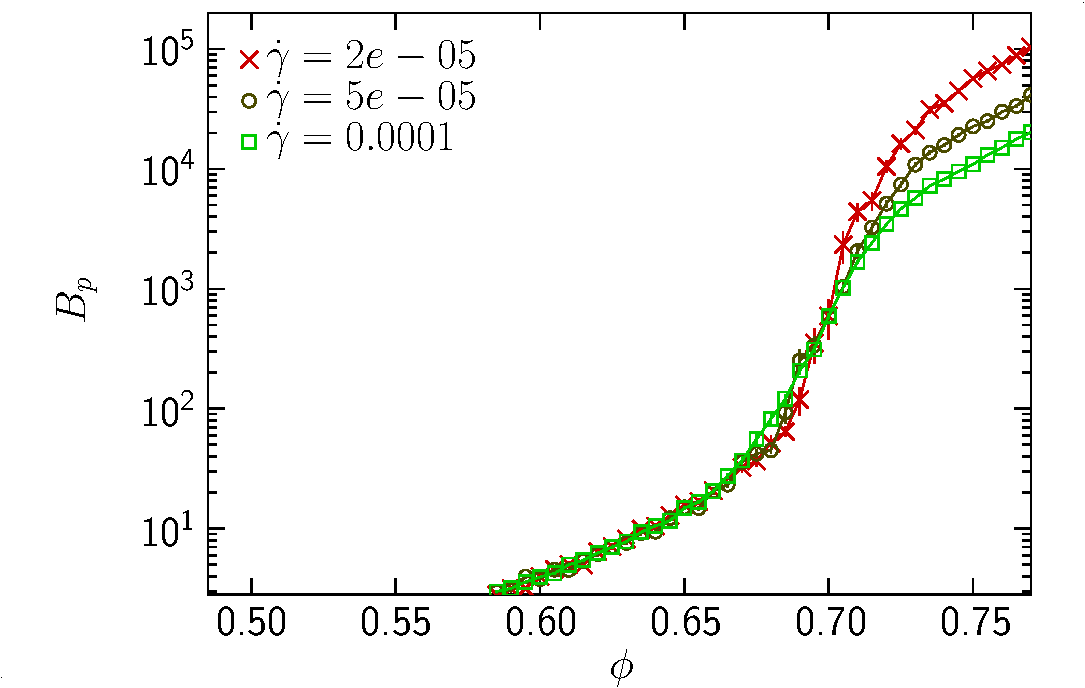
\includegraphics[width=\textwidth]{figures/figs/bp_0064_KDk500_Ml100_EL080}
        \caption{$\alpha=0.8$, $\phi_C\sim0.72$}
        \label{bp_0064_KDk500_Ml100_EL080}
    \end{subfigure}
    \hfill
     \begin{subfigure}[t]{0.49\textwidth}
        \centering
        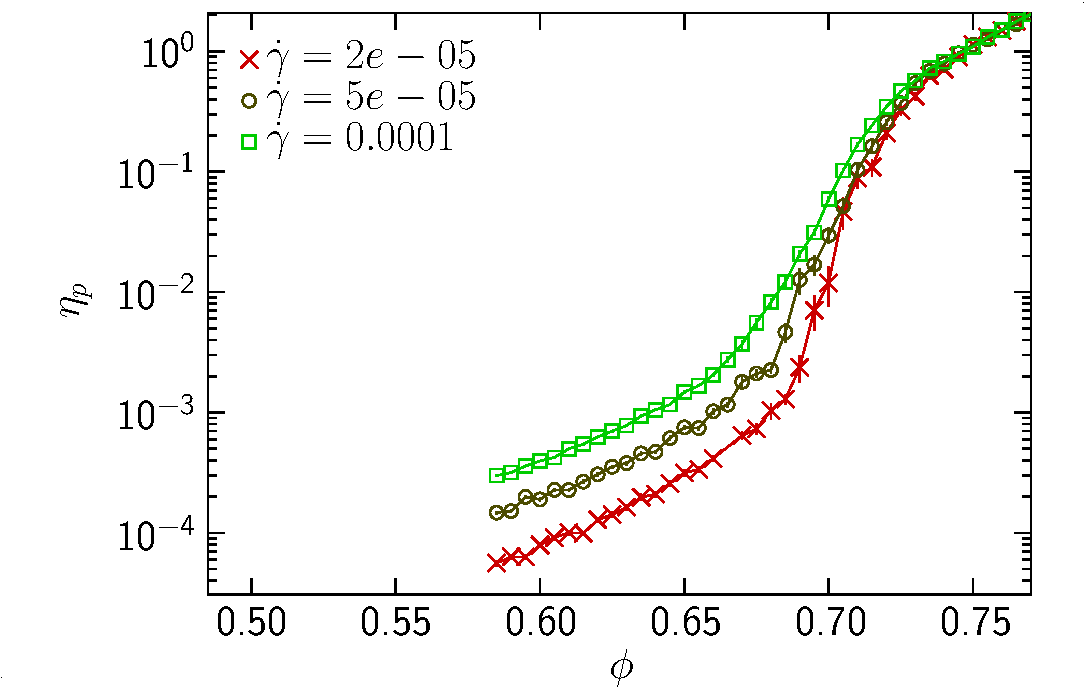
\includegraphics[width=\textwidth]{figures/figs/etap_0064_KDk500_Ml100_EL080}
        \caption{$\alpha=0.8$, $\phi_C\sim0.72$}
        \label{etap_0064_KDk500_Ml100_EL080}
    \end{subfigure}
    \caption{Coefficient de transport newtonien associé à la pression en fonction de la densité pour $\alpha=0.8$.}
\end{figure}
\vspace{-10pt}
Transition d’un régime bagnoldien (régime inertiel où les forces de dissipation sont négligeables) à un régime newtonien (régime sur-amorti où le terme inertiel du PFD est négligeable).

\end{frame}

\subsection{Comportement critique}

\begin{frame}{Écart au modèle de particules dures}

\begin{figure}[h!]
\centering
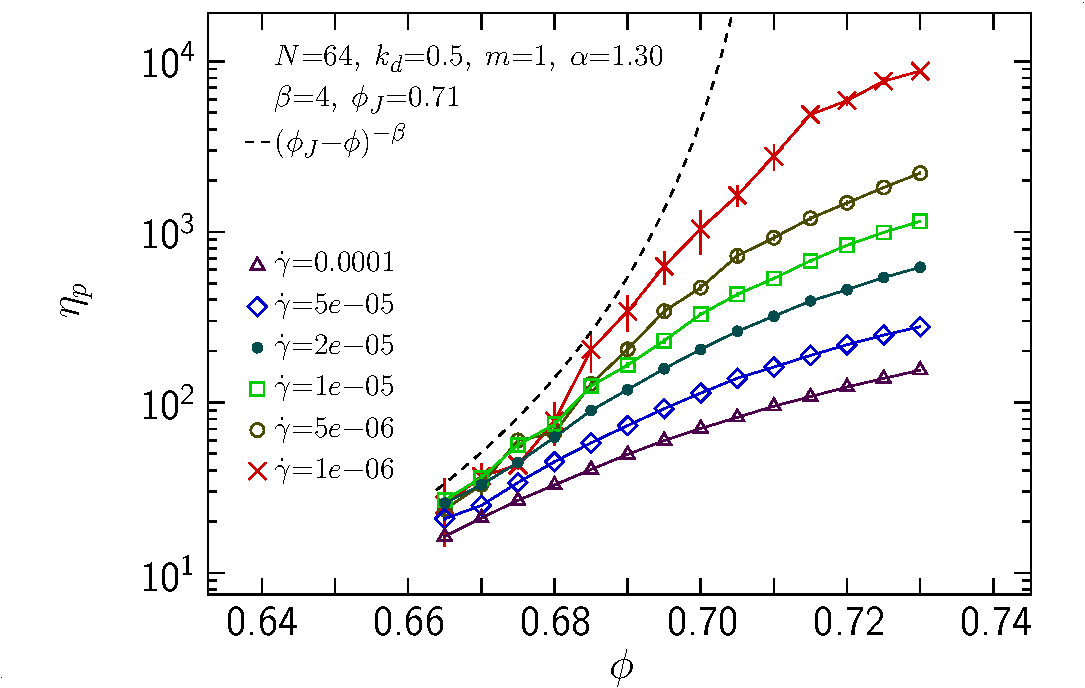
\includegraphics[width=0.6\textwidth]{figures/figs/etap-phi_0064_KDk500_Ml100_EL130}
\caption{Coefficient de transport newtonien associé à la pression en fonction de la densité pour $\alpha=1.3$.}
\end{figure}
\vspace{-10pt}
Écart au modèle de particules dures proche de la densité de jamming.
\begin{itemize}
\item[$\rightarrow$] L’écart est de moins en moins marqué pour des faibles taux de cisaillement.
\end{itemize}

\end{frame}

\begin{frame}{Divergence du coefficient de transport newtonien}

\begin{figure}[h!]
\centering
    \begin{subfigure}[t]{0.49\textwidth}
        \centering
        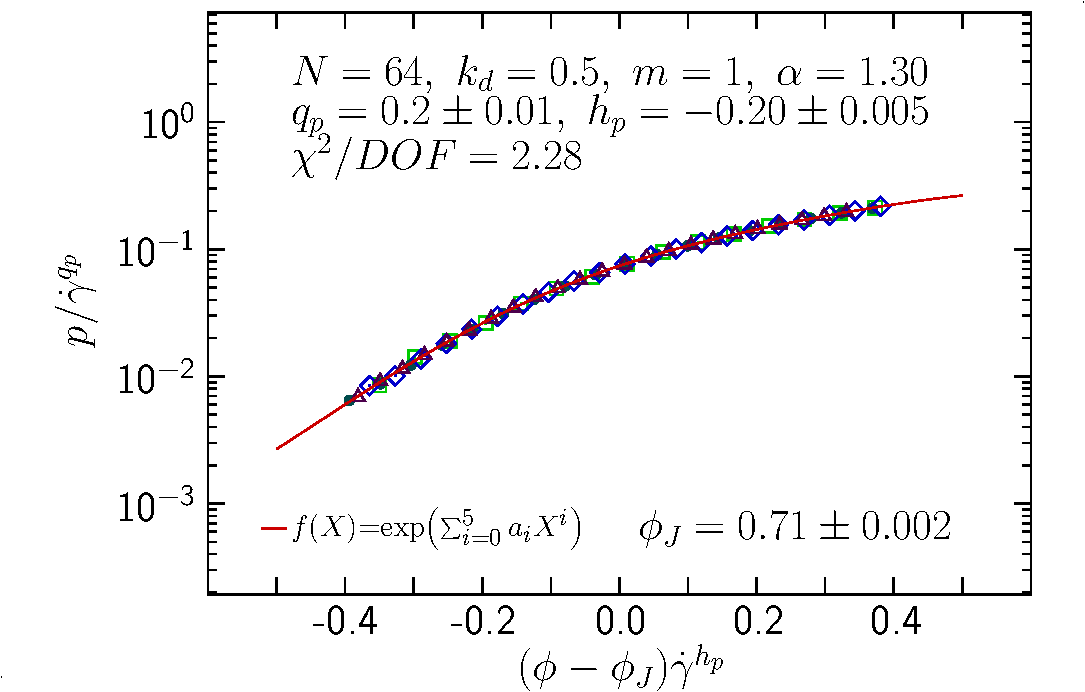
\includegraphics[width=\textwidth]{figures/figs/p-dphi-scale_0064_KDk500_Ml100_EL130}
    \end{subfigure}
    \hfill
    \begin{subfigure}[t]{0.49\textwidth}
        \centering
        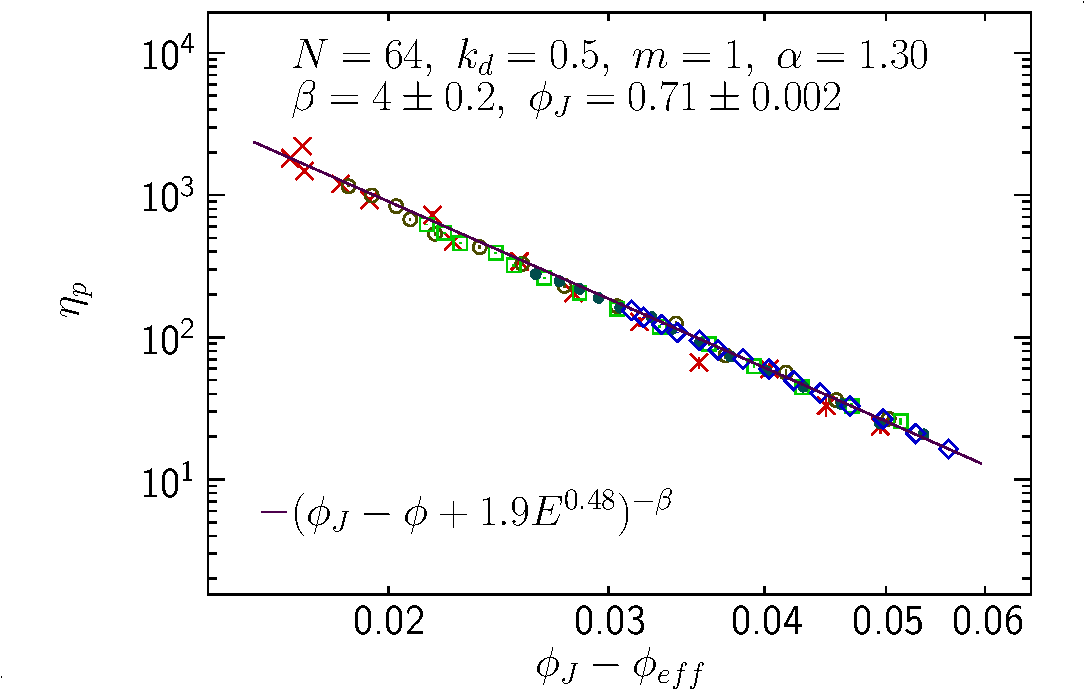
\includegraphics[width=\textwidth]{figures/figs/etap-phieff_graph_0064_KDk500_Ml100_EL130}
    \end{subfigure}
    \caption{Graphes de la pression pour $\alpha=1.3$.}
\end{figure}
\vspace{-10pt}
Notre hypothèse sur le comportement de la pression proche de la densité de jamming est correct comme l’indique ces graphes. Nous avons pris
\begin{align*}
\phi_{\text{eff}}(\phi,\dot{\gamma})\operatorname*{~=~}_{\phi\rightarrow\phi_J}\phi-cE(\phi,\dot{\gamma})^{1/y_E}
\end{align*}
permettant de faire la correspondance entre particules molles et dures proche de la transition de jamming.

\end{frame}

\begin{frame}{Densité de jamming et exposant critique}
\vspace{-10pt}
\begin{figure}[h!]
\centering
    \begin{subfigure}[t]{0.49\textwidth}
        \centering
        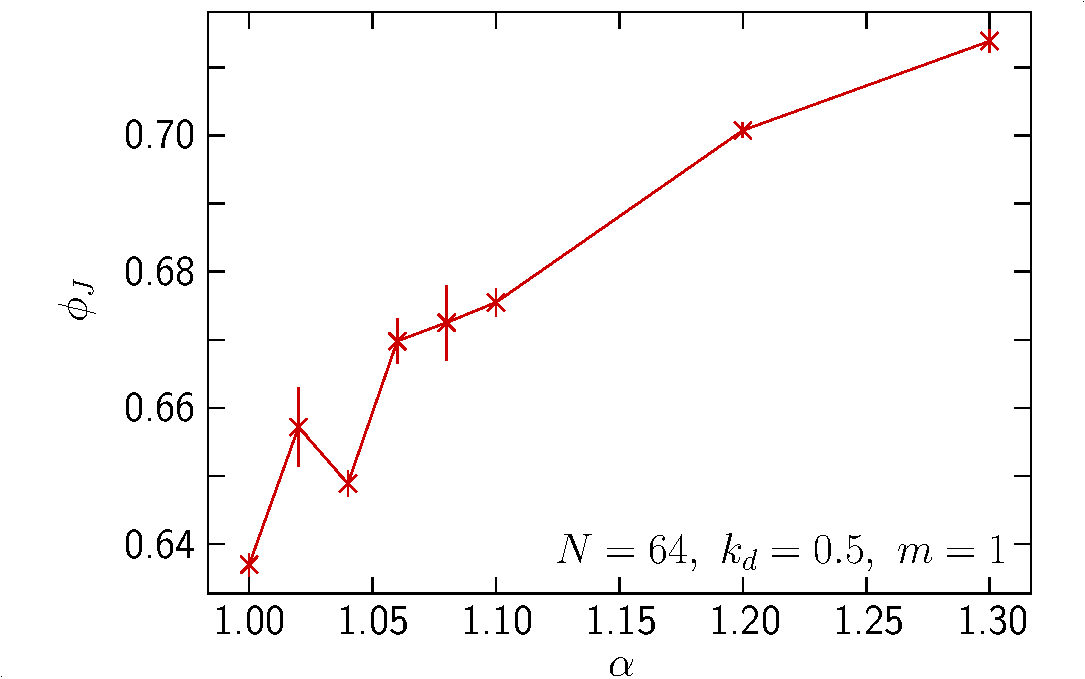
\includegraphics[width=\textwidth]{figures/figs/phij_alpha_0064_KDk500_Ml100}
    \end{subfigure}
    \hfill
    \begin{subfigure}[t]{0.49\textwidth}
        \centering
        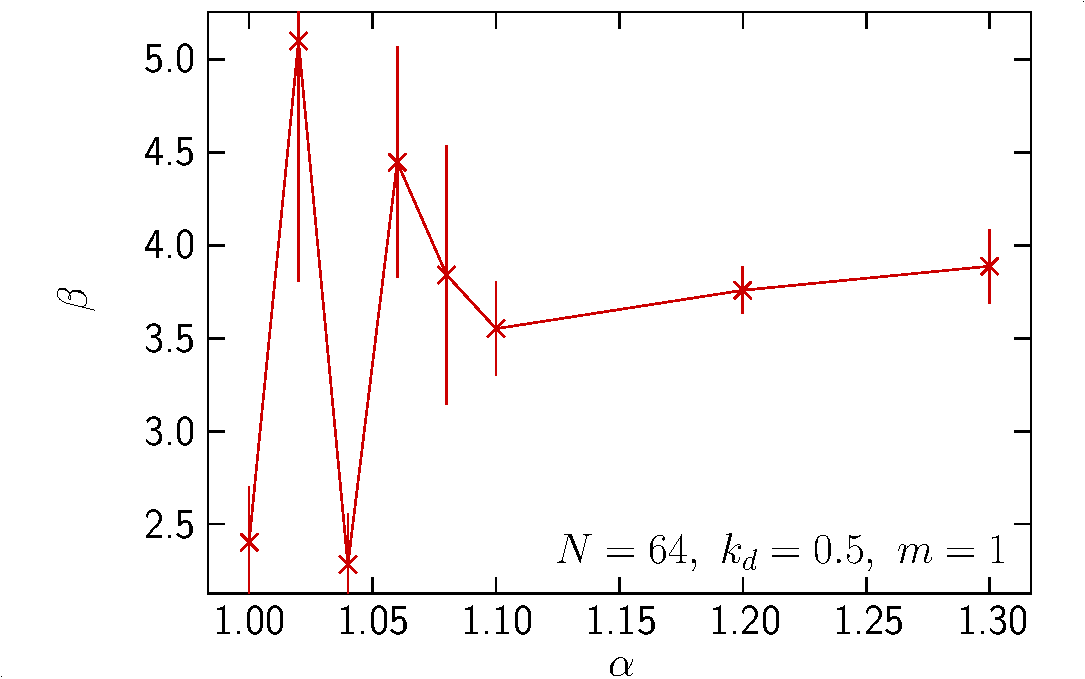
\includegraphics[width=\textwidth]{figures/figs/beta_alpha_0064_KDk500_Ml100}
    \end{subfigure}
    \caption{Densité de jamming $\phi_J$ et exposant critique $\beta$ en fonction du rapport d'aspect pour des particules allongées.}
\end{figure}
\vspace{-10pt}
La densité de jamming est une fonction croissante du rapport d’aspect pour des particules allongées.
\begin{itemize}
    \item[$\rightarrow$] Nous avons aussi observé que pour les rapports d’aspect $\alpha=0.9$ et $\alpha=0.8$ nous avions $0.7 < \phi_J(\alpha=0.9) < \phi_J(\alpha=0.8)$.
    \item[$\rightarrow$] Résultats cohérents avec les premiers travaux de Donev et al. (Science, 2004).
\end{itemize}

\end{frame}

\begin{frame}
Difficile de déterminer le comportent de $\beta$ en fonction d'$\alpha$, mais nous pouvons quand même affirmer qu’il devrait être proche de 4 pour des particules allongées.
\begin{itemize}
\item[$\rightarrow$] Il serait intéressant de savoir si toutes les particules allongées ont le même exposant $\beta$ (même classe d’universalité) et si cet exposant est une fonction discontinue du rapport d’aspect.
\end{itemize}
\end{frame}

\subsection{Orientation des particules}

\begin{figure}[h!]
\centering
    \begin{subfigure}[t]{0.32\textwidth}
        \centering
        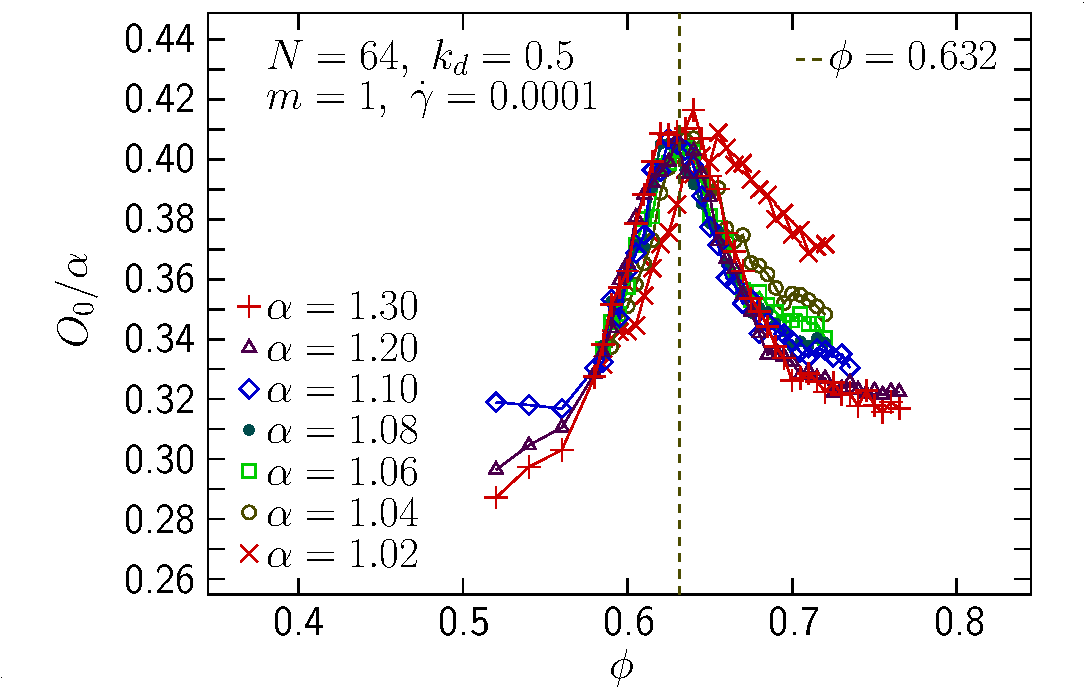
\includegraphics[width=\textwidth]{figures/figs/ori0al_phi_prolate_0064_KDk500_Ml100_GDh100}
    \end{subfigure}
    \hfill
    \begin{subfigure}[t]{0.32\textwidth}
        \centering
        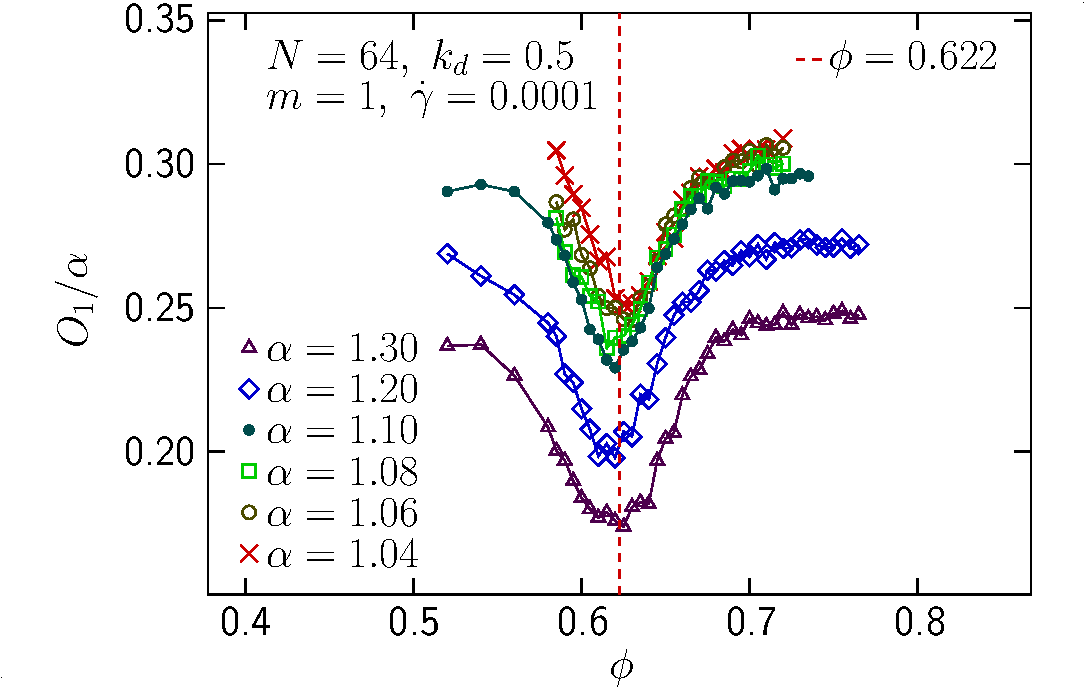
\includegraphics[width=\textwidth]{figures/figs/ori1al_phi_0064_KDk500_Ml100_GDh100}
    \end{subfigure}
    \hfill
    \begin{subfigure}[t]{0.32\textwidth}
        \centering
        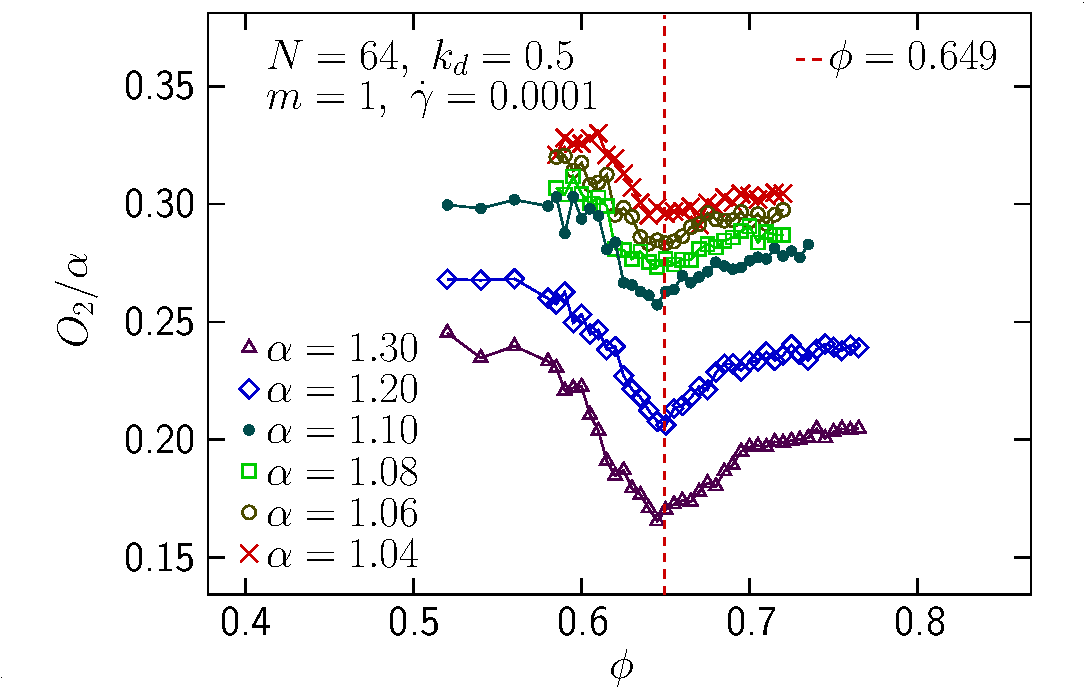
\includegraphics[width=\textwidth]{figures/figs/ori2al_phi_0064_KDk500_Ml100_GDh100}
    \end{subfigure}
	\caption{Moyenne du carré de la projection de l'axe de symétrie des particules selon différents axes en fonction de la densité.}
\end{figure}
\vspace{-20pt}
Les moyennes du carré de la projection de l’axe de symétrie des particules sur la direction de cisaillement attend un maximum pour une densité bien définie pour l’ensemble des $\alpha>1$ étudiés.
\begin{itemize}
    \item[$\rightarrow$] Ce maximum est $\appropto \alpha$.
\end{itemize}
Les moyennes du carré de la projection de l’axe de symétrie des particules sur les 2 autres axes correspondant atteignent des minimums à des densités toutes aussi bien définies pour l’ensemble des rapports d’aspects considérés.
\vspace{-17pt}
\begin{itemize}
    \item[$\rightarrow$] Les 3 densités correspondant à des extrema du carré de ces projections sont toutes différentes.
    \item[$\rightarrow$] Les minima ne sont pas proportionnels au rapport d’aspect.
\end{itemize}

\begin{frame}{Corrélation de l'orientation}

\begin{figure}[h!]
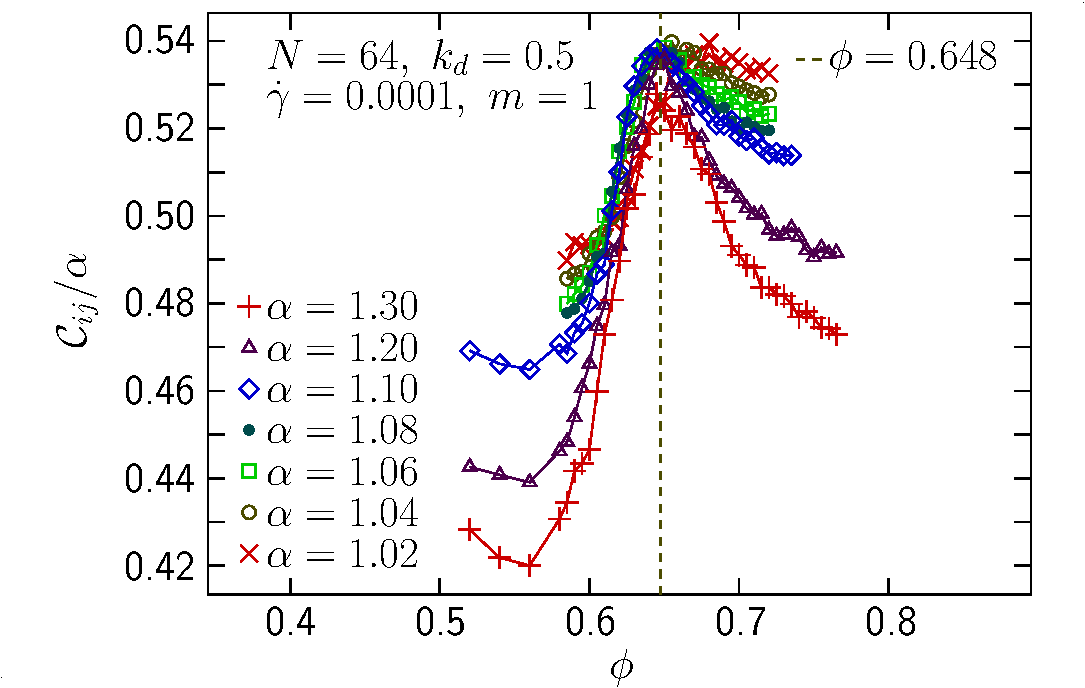
\includegraphics[width=0.6\textwidth]{orijal_phi_prolate_0064_KDk500_Ml100_GDh100}
\caption{Corrélation de l'orientation des particules en fonction de la densité.}
\end{figure}
\vspace{-10pt}
La fonction de corrélation de l’orientation attend aussi un maximum à une densité bien définie pour les rapports d’aspect considérés, proche de la densité pour laquelle le minima de la projection sur l’axe 2 apparaissait.
\begin{itemize}
\item[$\rightarrow$] Ce maximum est proportionnel au rapport d’aspect.
\end{itemize}

\end{frame}

\subsection{Temps de relaxation}

\begin{frame}{Décroissance exponentielle de la pression}

\begin{figure}[h!]
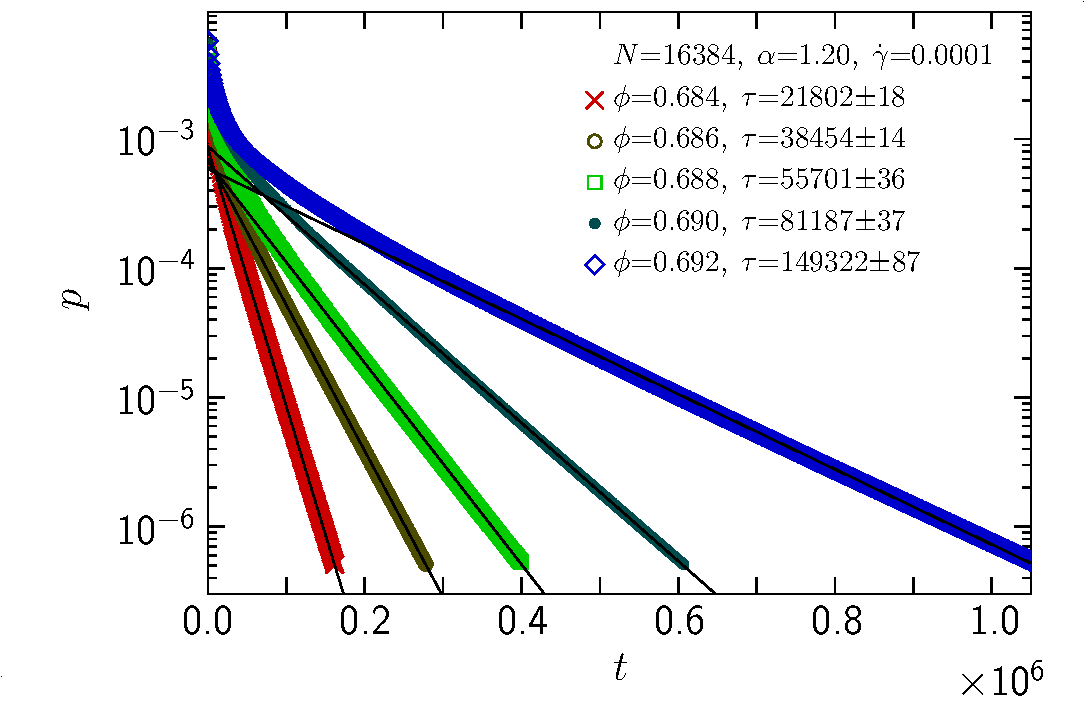
\includegraphics[width=0.6\textwidth]{pe_t_16384_EL120_GDh100}
\caption{Pression en fonction du temps pendant la phase de relaxation.}
\end{figure}
Nous observons bien une décroissance exponentielle de la pression pendant la période de relaxation et que le temps de relaxation est une fonction décroissante de l’écart à la densité de jamming.

\end{frame}

\begin{frame}{Densité de jamming et exposant critique}

\begin{figure}[h!]
\centering
    \begin{subfigure}[t]{0.49\textwidth}
        \centering
        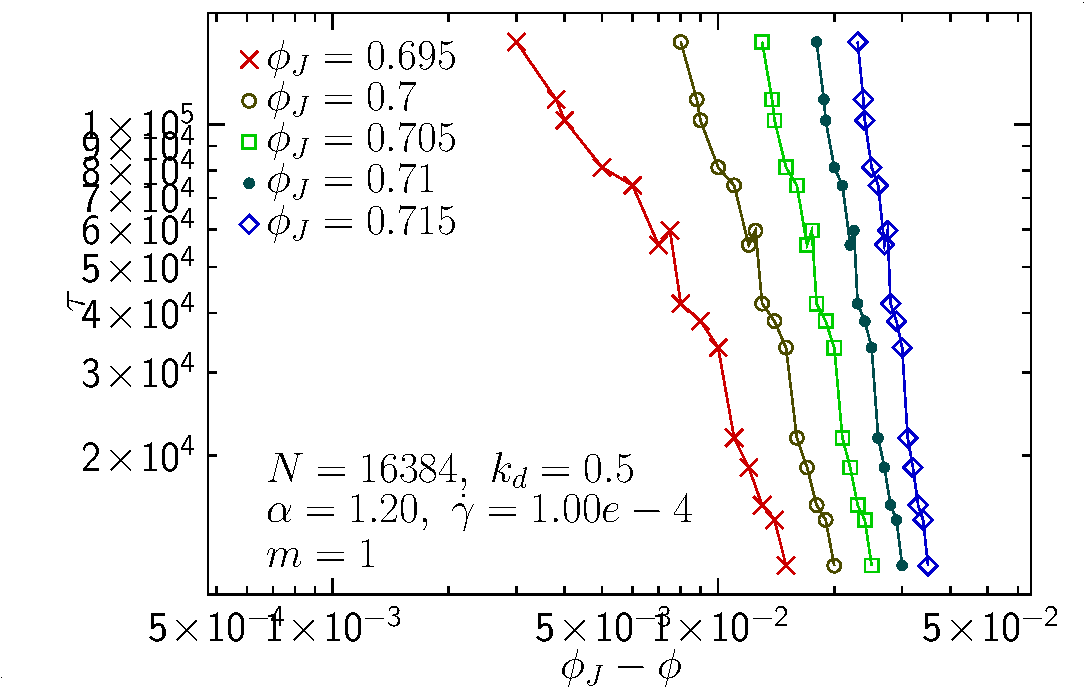
\includegraphics[width=\textwidth]{figures/figs/tau_dphi_16384_GDh100_EL120}
    \end{subfigure}
    \hfill
    \begin{subfigure}[t]{0.49\textwidth}
        \centering
        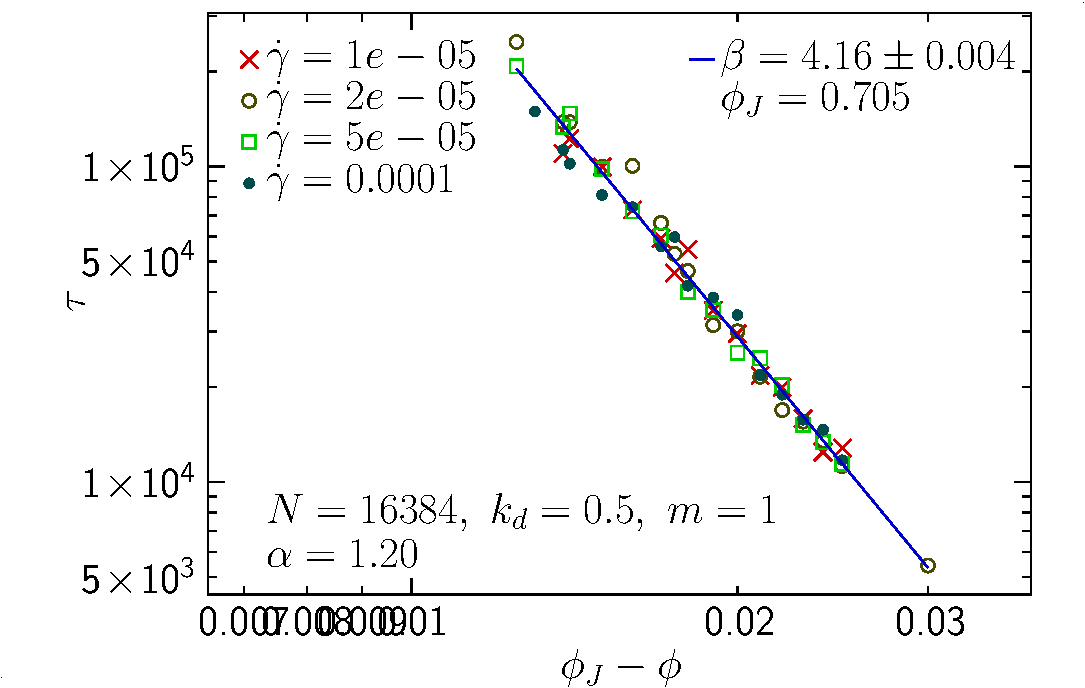
\includegraphics[width=\textwidth]{figures/figs/tau_dphi_16384_PJ70500_EL120}
    \end{subfigure}
    \caption{Détermination graphique de l'exposant critique $\beta$ et de la densité de jamming $\phi_J$.}
\end{figure}
Nous déterminons la densité de jamming de manière graphique et le coefficient beta par régression linéaire.
\begin{itemize}
    \item[$\rightarrow$] La méthode est efficace.
\end{itemize}

\end{frame}

{
\makeatletter % to change template
    \setbeamertemplate{headline}[default] % not mandatory, but I though it was better to set it blank
    \def\beamer@entrycode{\vspace*{-\headheight}}
\begin{frame}{Conclusion}

\begin{itemize}
\item Nos premiers résultats sont en accord avec la littérature existante : accord quantitatif avec les papiers de Olsson et al. pour les particules sphériques, accord qualitatif avec Donev et al. (Science, 2004) pour les particules sphéroïdales.
\item Nous avons observé que la densité de transition rhéologique était indépendante du rapport d’aspect.
\item Pour les systèmes de particules sphéroïdales étudiés, $\phi_J$ est très élevée (proche de la densité de la CFC pour des sphères).
\begin{itemize}
\item[$\rightarrow$] Il serait intéressé de savoir quel est la densité de l’ensemble le plus ordonné de telles particules pour savoir si nous pouvons observer une cristallisation.
\end{itemize}
\item L’observation des projections des axes de symétries des particules a montré que ces fonctions atteignaient des extrema à des densités bien définies ne correspondant ni à la transition rhéologique, ni à la transition de jamming.
\begin{itemize}
\item[$\rightarrow$] Ce phénomène doit être plus étudié.
\end{itemize}
\end{itemize}

\end{frame}
}

{
\makeatletter % to change template
    \setbeamertemplate{headline}[default] % not mandatory, but I though it was better to set it blank
    \def\beamer@entrycode{\vspace*{-\headheight}}
\begin{frame}{Conclusion}

\begin{itemize}
\item Il serait intéressant d’étudier le nombre de contacts à la transition de jamming pour confirmer les hypothèses d’hypostaticité de Donev (PRE, 2007), pour des ensembles de particules ellipsoïdales.
\item Il serait aussi intéressant de déterminer si l’exposant critique beta est dépendant du rapport d’aspect et si les ensembles de particules ellipsoïdales pourraient ainsi être décrits par une même classe d’universalité.
\end{itemize}

\end{frame}
}

\end{document}
